\section{\acl{HMM}}
\label{mainsec:hmm}
\textit{Paul Pasler, Sebastian Rieder}

Das \acl{HMM} ist ein stochastisches Modell für sequentielle Daten und wird vor allem in der Spracherkennung und in der Bioinformatik eingesetzt.

In den folgenden beiden Abschnitten werden die Entstehung und Konzepte der \acl{MK} und des \acl{HMM} aufgezeigt.
Abschnitt \ref{sec:preproc} befasst sich mit der Aufbereitung der Daten für das Training und die Klassifizierung der Gesten.
Die Implementierung und Anwendung des \acl{HMM} werden im Abschnitt \ref{sec:impl} näher erläutert. Im letzten Abschnitt werden die Ergebnisse 
evaluiert und ein Fazit mit Ausblick gezogen.  
 
  %%%%%%%%%%%%%%%%%%
  %  MARKOV-KETTE  % 
  %%%%%%%%%%%%%%%%%%  
\subsection{\acl{MK}} \label{sec:chain}
Grundlage des \acl{HMM} war die vom russischen Mathematiker Andrej Andrejewitsch Markov 
(1856 - 1922, siehe \cite{markov1913}) entwickelte \acl{MK}. Zu Beginn des
20. Jahrhunderts beschäftigte er sich als erster mit einer statistischen Beschreibung von Zustands- und Symbolfolgen. 
Er führte eine statistische Analyse der Buchstabenfolge des Textes ``Eugen Onegin'' von Alexander 
Pushkin.

Eine \acl{MK} beschreibt einen zeit-diskreten Prozess \((X_t)_{t\in\mathbb{N}_0}\) mit  \(m\) abzählbaren Zuständen \(S\) \cite{stochMod}.
Weiterhin wird sie als stationär bezeichnet, wenn alle Wahrscheinlichkeiten unabhängig von der Zeit sind.
Da die Verteilung der Zufallsvariablen nur von den vergangenen Zuständen abhängt, gilt eine \acl{MK} als kausal \cite[48]{mmmFink}.
Wichtig für eine \acl{MK} ist die sog. Markov-Eigenschaft:
\[ P (X_{t+1} = s_{t+1} | X_0 = s_0, \ldots , X_{t-1} = s_{t-1}, X_{t} = s_{t}) \]
\[ = P ( X_{t+1} = s_{t+1} | X_{t} = s_{t} ) \] \\
Genügt eine \acl{MK} dieser Eigenschaft, wird sie als ``einfach'' oder \acl{MK} 1. Ordnung bezeichnet.
Anders ausgedrückt beschreibt die Markov-Eigenschaft die Gedächtnislosigkeit des Prozesses, da der Folgezustand nur vom direkten Vorgänger abhängt.

Als Übergangswahrscheinlichkeit bezeichnte man die bedingte Wahrscheinlichkeit \(P ( X_{t+1} = s_{t+1} | X_{t} = s_{t} ) \), sodass auf 
den aktuellen Zustand \( s_{t}\) der Nachfolgezustand \( s_{t+1}\) folgt. Diese Wahrscheinlichkeiten werden üblicherweise zu einer Übergangsmatrix zusammengefasst: 
\[ A = [a_{ij}] =
\begin {bmatrix} 
  a_{00}&\cdots&a_{0m} \\
  \vdots&\ddots&\vdots \\
  a_{m0}&\cdots&a_{mm}
 \end {bmatrix} \forall i, j \in S \]
Da es sich um Wahrscheinlichkeiten handelt, muss sich die Summe jeder Reihe zu Eins addieren. \\

Weiterhin benötigt der Prozess einen Vektor für den Anfangzustand \( t = 0 \):
\[ \Pi = [ \pi_i] = [ P (X_0 = i) ] , i \in S \]

So lässt sich eine Markov-Kette durch Zustandsraum \(S\), den Übergangsmatrix \( A \) und einen Anfangszustand \( \Pi \) definieren.
Veranschaulichen lässt sich eine Markov Kette als gerichtetes Zustandsdiagramm (Abb. \ref{fig:simple_mc}) mit den Zuständen \(S\) und 
mit den Übergangswahrscheinlichkeiten \(X_i\) an den Kanten
\begin{figure}[htbp] \centering
    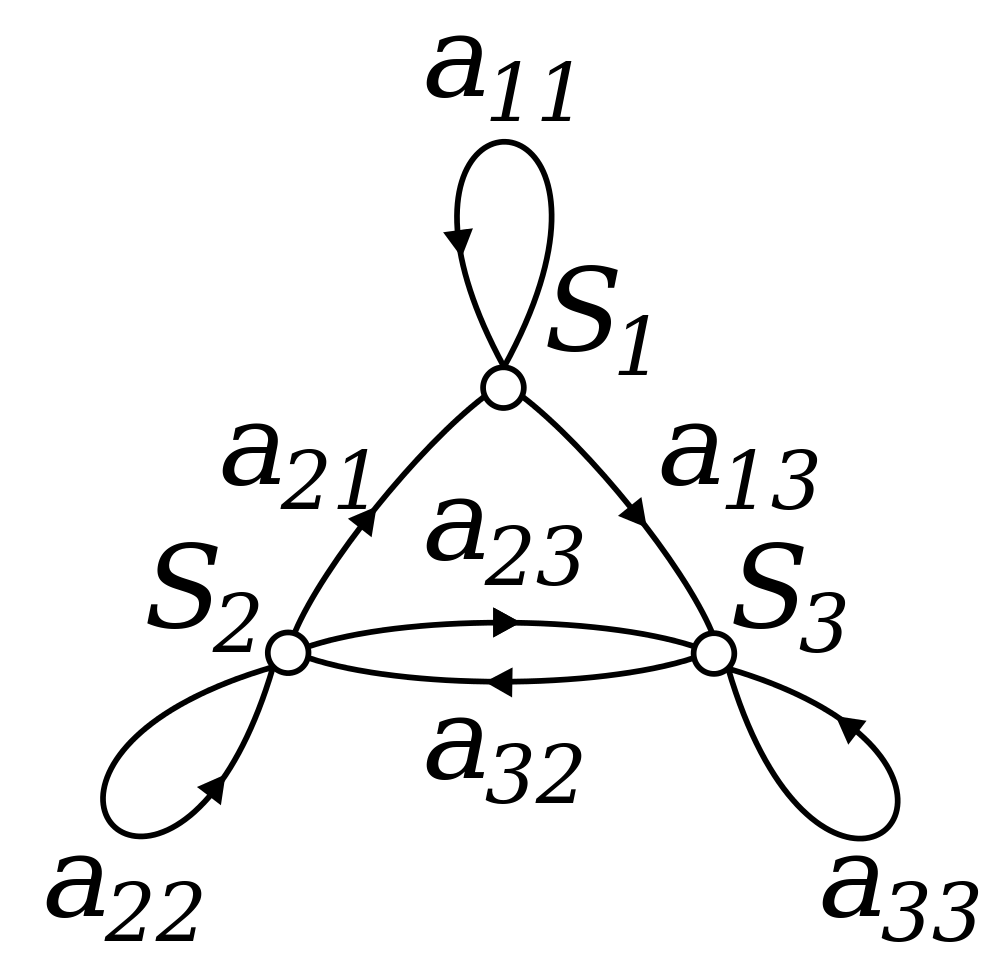
\includegraphics[width=0.33\textwidth]{markov/simple_mc.png}
    \caption{Einfaches Zustandsdiagramm einer \acl{MK} (de.wikipedia.org/wiki/Markow-Kette)}
    \label{fig:simple_mc}
\end{figure}
Die Wahrschinlichkeit für \( k \)-Schritte lässt sich so ausrechnen: 
\[ X_k = X_{k-1} A = X_0 A^k \] 


\textbf{Beispiel} \acl{MK} für die Wahrscheinlichkeit des Wetters \\
(Quelle: en.wikipedia.org/wiki/Examples\_of\_Markov\_chains) \\
Im folgenden Beispiel soll aufgrund des aktuellen Wetters auf das Wetter der folgenden Tage geschlossen werden.
Das Wetter kann entweder ``sonnig'' oder ``regnerisch'' sein, zu Beginn (Tag 0, \( t = 0 \)) des Experiments ist es ``sonnig''.
Die Wahrscheinlichkeit, dass auf ``sonnig'' wieder ``sonnig'' folgt, liegt bei 90\% (``regnerisch'' = 1 - ``sonnig'' = 10\%). 
Nach ``regnerisch'' liegt die Wahrscheinlichkeit jeweils bei 50\%.  
\begin{figure}[htbp] \centering
    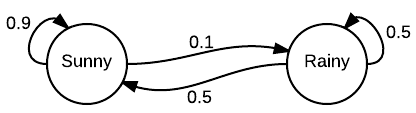
\includegraphics[width=0.33\textwidth]{markov/simple_mc_example.png}
    \caption{ Gerichteter Zustandsgraph der modellierten Wetter-\acl{MK} }
    \label{fig:simple_mc_example}
\end{figure}

Zustände \( S = [``sonnig'', ``regnerisch'']\) \\
Anfangszustand ``sonnig'' \( \Pi = X_0 = [1 , 0] \) \\
Übergangsmatrix \( \begin {bmatrix} 0.9&0.1\\0.5&0.5 \end {bmatrix} \)

Nun kann die Wahrscheinlichkeit für das Wetter an Tag 1 berechnet werden über: \\
\[ X_1 = X_0 * A = [ 1, 0 ] \begin {bmatrix} 0.9&0.1\\0.5&0.5 \end {bmatrix} = [ 0.9, 0.1] \]

Für Tag 2:\\
\[ X_2 = X_1 A = X_0 A^2 = [ 1, 0 ] \begin {bmatrix} 0.9&0.1\\0.5&0.5 \end {bmatrix}^2 = [ 0.86, 0.14] \] 

Verallgemeinert für Tag k bedeutet das: 
\[ X_k = X_{k-1} A = X_0 A^k = [ 1, 0 ] \begin {bmatrix} 0.9&0.1\\0.5&0.5 \end {bmatrix}^k \] 


  %%%%%%%%%%%%%%%%%%
  %  HIDDEN-MARKOV  % 
  %%%%%%%%%%%%%%%%%%
\subsection{\acl{HMM} und \acl{GMM}}  \label{sec:hmm}
Der amerikanischen Mathematiker Leonard E. Baum (* 1931) und andere Autoren entwickelten auf Basis der \acl{MK} Ende der 
sechziger Jahre das \acl{HMM}. Erste \acl{HMM}-Applikationen wurden zur Spracherkennung und später auch in der Bioinformatik 
zur Analyse von Nukleotid- und Proteinsequenzen eingesetzt. 

Ein \acl{HMM} erweitert eine \acl{MK} um eine weiteren Zufallsprozess und ist
somit ein zweistufiger stochastischer Prozess \cite[67]{mmmFink}. Hierfür wird
jedem Zustand der \acl{MK} eine Ausgabe bzw. Emission zugeordnet dessen
Wahrscheinlichkeitsverteilung einzig vom aktuellen Zustand abhängig ist. Die
Emissionen sind die einzigen beobachtbaren Zustände des \acl{HMM}. Der Rest
ist sozusagen 'versteckt' woher sich auch der Name des Models ableitet. Eine
Folge von Emissionen wird auch Observationsfolge genannt.


Das \acl{HMM} wird definiert durch \cite[68]{mmmFink}:\\ 
\( \lambda = (S;V;A;B;\pi)\)
\begin{itemize}
     \item Endlich Menge von Zuständen \\
           \( S = \{ s | 1 <= s <= N \} \)
     \item Alphabeth der Emissionen \\
           \( V = \{ v | 1 <= v <= M \} \)
     \item Matrix der Zustandsübergangswahrscheinlichkeiten \\
           \( A = \{ a_{ij} | a_{ij} = P(S_t = j | S_{t-1} = i) \} \)
     \item Matrix der Emissionsverteilung \\
           \( B = \{ b_{jk} | b_{jk} = P(O_t = o_k | S_t = j) \} \) bzw. \( B =
           \{ b_{j}(x) | b_{j}(x) = p(x|S_t = j) \} \)
     \item Vektor von Zustandsstartwahrscheinlichkeiten \\
           \( \pi = \{ \pi_i | \pi_i = P(S_1 = i) \} \) 
\end{itemize}

Die Emissionsmodellierung ist hierbei vom Kontext der Problemstellung abhängig.
Wird das \acl{HMM} zum Beispiel bei der Analyse von biologischen Sequenzen,
sprich einem diskreten Symbolinventar, angewendet, wird ein diskretes
Emissionsmodel genutzt. Man spricht hierbei auch von einem diskreten \acl{HMM}.
Wenn dieses Model zur verarbeitung von Signalen verwendet werden soll erfordert
dies in der Vorverarbeitung der Daten einen Quantisierer der die
kontinuerlichen Merkmale in eine diskrete Observationsfolge überführt. 

Gänger ist es hierfür kontinuierliche \acl{HMM}'s zu nutzen. Hierbei wird eine
Emissionsmodelierung auf Basis kontinuierlicher Dichtefunktionen genutzt die
kontinuierliche Observationen im \(\mathbb{R}^n\) verarbeitet.\\ 
\( B =\{ b_{j}(x) | b_{j}(x) = p(x|S_t = j) \} \)
Zur behandlung kontinuerlicher Verteilungen mit mehreren komplexen
Häufigkeitsgebieten werden approximatische Verfahren genutzt. Die verbreiteste
Technik besteht aus der Verwendung von Mischverteilungen auf der Basis von
Gauß-Dichten (\acl{GMM}). Man kann nämlich zeigen, dass sich jede allgemeine
kontinuierliche Verteilung \(p(x)\) durch eine Linearkombination von i.a. unendlich vielnen
Basis-normalverteilungen beliebig genau approximieren lässt\cite[69]{mmmFink}:\\
\begin{equation}
\begin{multline}
p(x) \hat{=} \sum_{k=1}^\infty c_{k} N(x|\mu_{k},K_{k}) \\
approx \sum_{k=1}^M c_{k} N(x|\mu_{k},K_{k})  
\end{multline}
\end{equation}

Das Konzept des \acl{HMM} kann laut \cite{rabiner} in drei Problemstellungen eingeteilt werden:
\begin{itemize}
  \item Evaluierungsproblem: 
  \item Dekodierungsprobem: Finde interne Abläufe für eine gegebene Observationsfolge
  \item Trainingsproblem: Finde Modellparameter für gegebene Beispieldaten
\end{itemize}




Um das Training und die Klassifizierung möglichst genau und perfomant umzusetzen, 
ist es notwendig die aufgenommenen Daten auzubereiten, dies ist Thema des nächsten Abschnitts


  %%%%%%%%%%%%%%%%%%%
  %  PREPROCESSING  % 
  %%%%%%%%%%%%%%%%%%%
\subsection{Datenaufbereitung} \label{sec:preproc}
Ziel der Vorverarbeitung ist es die Daten zu normieren und die Datenmenge zu reduzieren, um das Trainingergebnis bzw. Performance zu verbessern.
Weiterhin werden relevante Werte bzw. Werte mit hohem Informationsgehalt einer Geste aus der Aufnahme vertärkt. \\


\textbf{Rohdaten} \\
Eine Aufnahme wird beschrieben durch ein zwei-dimensionales Array aus 32 Frames mit jeweils 64 Frequenzwerten.
Im Ruhezustand bildet sich ein Normalsignal mit einem Peak um die ausgesendete Frequenz (18.500hz, siehe Abb. \ref{fig:data_raw}).

\begin{figure}[htbp] \centering
    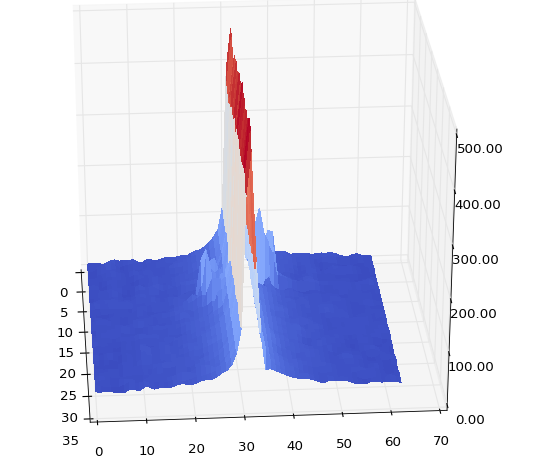
\includegraphics[width=0.4\textwidth]{markov/data_raw.png}
    \caption{Rohdaten direkt vom Recorder (\acl{RLO} Geste) mit gefundener Gestenmitte (Roter Punkt)}
    \label{fig:data_raw}
\end{figure}

\textbf{Verarbeitung}\\
Da sich Änderungen durch eine Bewegung sehr Nahe am Normalignal liegen, werden die Daten im 
Frequenzbereich von 18.000hz bis 19.000hz betrachtet, die Daten vermindern sich von 64 auf 16 Werte pro Frame. 
Dazu wird jede Geste auf einem Intervall von 0 bis 1 normalisiert (Geteilt durch den jeweiligen Maximalwert der Geste) und 
auf zwei Nachkommstellen gerundet. 
Alle Werte unterhalb eines Schwellwerts (0.15) werden zudem abgeschnitten, um niedrig amplitudiges Rauschen zu vermindern. 
So wird im Idealfall nur das gesendete Signal und Frequenzänderungen durch eine Bewegung dargestellt.

Das Normalsignal mit einer hohen Amplitude (Normalisiert im Bereich zwischen 0.8 und 1.0) birgt einen geringen Informationsgehalt, 
eine Frequenzverschiebung durch eine Geste ist deutlich interessanter, jedoch schwächer in der Amplitude (Zwischen 0.15 und 0.5).
Darum wird werden niedrige Amplitudenwerte \( x \) verstärkt und hohe abgeschwächt. Folgende Funktion wird auf alle Werte angewendet: \\
\( f(x) = 2.8 \cdot ( x - 1.15 )^2 + 0.75 \) (Verlauf siehe Abb. \ref{fig:funktion})
\begin{figure}[htbp] \centering
    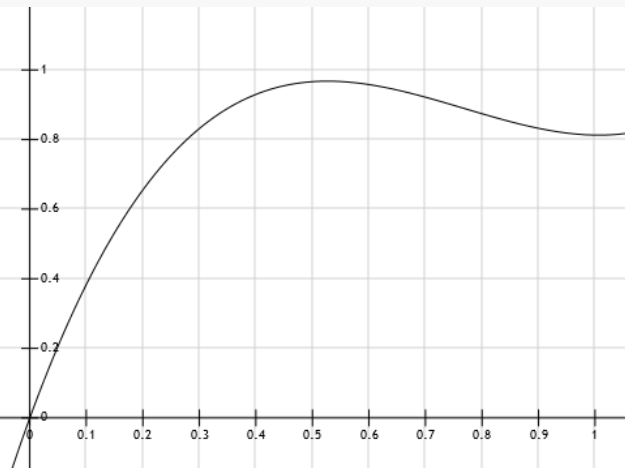
\includegraphics[width=0.4\textwidth]{markov/funktion.png}
    \caption{Kubische Parabel zur Verstärkung / Abschwächung der Amplitude}
    \label{fig:funktion}
\end{figure}

Nach der Vorverarbeitung sind die Frequenzbereiche links und rechts neben dem Normalsignal deutlicher herausgearbeitet (Siehe Abb. \ref{fig:data_preproc}).  

\begin{figure}[htbp] \centering
    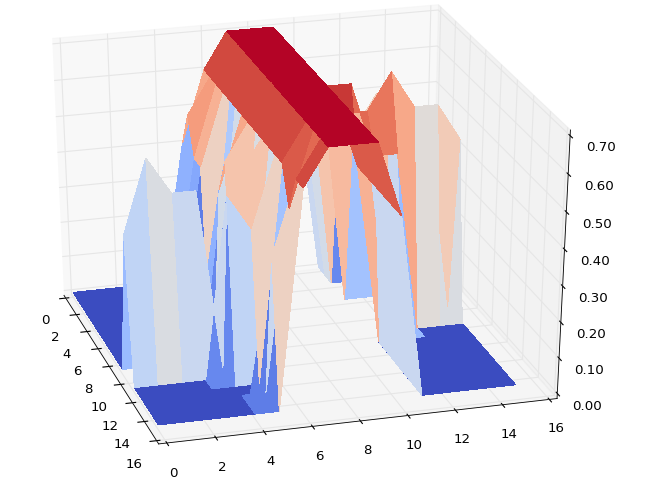
\includegraphics[width=0.4\textwidth]{markov/data_preproc.png}
    \caption{Daten nach der Vorverarbeitung (\acl{RLO} Geste)}
    \label{fig:data_preproc}
\end{figure}

\textbf{\acl{GMM}} \\
Aus den Vorverarbeiteten Daten werden Gauß’sche Mixtur Modelle berrechnet

\begin{figure}[htbp] \centering
    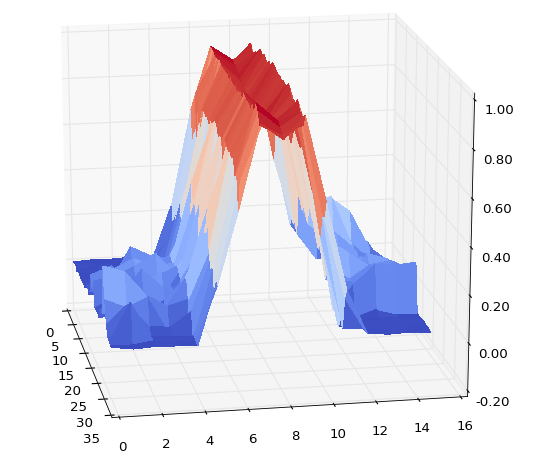
\includegraphics[width=0.4\textwidth]{markov/data_gmm.png}
    \caption{Sampledaten aus dem trainierten \acl{GMM} (\acl{RLO} Geste)}
    \label{fig:data_gmm}
\end{figure}

  %%%%%%%%%%%%%%%%%%%%%
  %  IMPLEMENTIERUNG  % 
  %%%%%%%%%%%%%%%%%%%%%
\subsection{Implementierung}  \label{sec:impl}
Wir haben uns für die scipy HMM implementierung entschieden. 
Genutzt wird ein \acl{HMM} mit \acl{GMM} entschieden.


  %%%%%%%%%%%%
  %  RESULT  % 
  %%%%%%%%%%%%
\subsection{Evaluation und Fazit}  \label{sec:result}
Das Hidden Markov Modell eignet sich grundsätzlich sehr gut für die gestellte Aufgabe. Da es mit sequenzielle Daten (Frames) umgehen 
kann und ursprünglich für die Spracherkennung entwickelt wurde. Ob nun aus einem Tonsignal (versteckte Zustände) ein Wort oder 
eine Geste (Emissionen) erkannt werden soll, ist vom Vorgehen ähnlich. Ein Vorteil ist zudem, dass die Ausführungsgeschwindigkeit
 der Geste, bei geeigneter Aufnahmelänge, die Klassifizierung nicht unbedingt beeinflusst, da dann länger im selben versteckten 
 Zustand verblieben wird.
Ein Nachteil dieser Methode ist, dass keine absoluten Klassifizierungen durchgeführt werden können. Es werden nur Wahrscheinlichkeiten für alle möglichen Klasse berechnet. So muss entschieden werden, ob die Wahrscheinlichkeit für eine Klasse hoch genug ist, sodass diese als Geste identifiziert werden kann.
